\chapter{Layers in NN models}

\begin{enumerate}
    \item \url{https://pytorch.org/docs/stable/nn.html#linear-layers}
    \item \url{https://www.tensorflow.org/api_docs/python/tf/keras/layers}
\end{enumerate}

%%%%%%%%%%%%%%%%%%%%%%%%%%%%%%%%%%%%%%%%%%%%%%%%%%%%%%%%%%%%

\section{Linear Layer/ Dense Layer \cite{pytorch-Linear,gfg-convolutional-neural-network-cnn-in-machine-learning}}\label{nn: Linear Layer/ Dense Layer}

\begin{enumerate}
    \item These layers are responsible for making predictions based on the high-level features learned by the previous layers. 
    
    \item They connect every neuron in one layer to every neuron in the next layer.
    
    \item Applies a linear transformation to the incoming data: $\mathbf{y=xA^\top+b}$.
\end{enumerate}


%%%%%%%%%%%%%%%%%%%%%%%%%%%%%%%%%%%%%%%%%%%%%%%%%%%%%%%%%%%


\section{(Linear) Convolution Layer \cite{gfg-convolutional-neural-network-cnn-in-machine-learning}}\label{nn: Convolution Layer}

SEE: \fullref{function: Convolution}

\begin{table}[h]
    \begin{minipage}{0.44\linewidth}
        \begin{figure}[H]
            \centering
            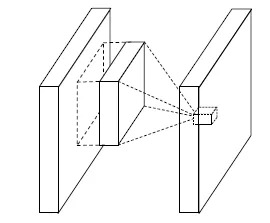
\includegraphics[width=\linewidth, height=4cm, keepaspectratio]{Pictures/layers/conv-layer-linear.jpg}
            \caption{(Linear) Convolution Layer \cite{medium/towardsdatascience.com/review-nin-network-in-network-image-classification-69e271e499ee}}
        \end{figure}
    \end{minipage}
    \hfill
    \begin{minipage}{0.54\linewidth}
        \begin{customTableWrapper}{1.5}
        \begin{table}[H]
            \begin{tabular}{l p{5.5cm}}
                $n_h$ and $n_w$ & size of input $n_h \times n_w$ \\
                $n^{out}_h$ and $n^{out}_w$ & size of output $n^{out}_h \times n^{out}_w$ \\
                $p_h$ and $p_w$ & padding $p_h/2 \times p_w/2$ \\
                $k_h$ and $k_w$ & kernel/ filter $k_h \times k_w$\\
                $s_h$ and $s_w$ & stride $s_h \times s_w$ \\

                \hline

                $n_f^{prev}$ or $c_i$ & number of channels in image/ num of filters in previous layer \\
                $n_f^{curr}$ or $c_o$ & number of filters in current layer \\
                
            \end{tabular}
        \end{table}
        \end{customTableWrapper}
    \end{minipage}
\end{table}

\begin{enumerate}[itemsep=0.2cm]
    \item These layers apply convolutional operations to input images, using filters (also known as kernels) to detect features such as edges, textures, and more complex patterns. 
    
    \item Convolutional operations help preserve the spatial relationships between pixels.

    \item[] output dimensions: 
    $
        \hfill
        n^{out}_h=\dfloor{\dfrac{n_\textrm{h}-k_\textrm{h}+p_\textrm{h}+s_\textrm{h}}{s_\textrm{h}}}
        \hfill 
        n^{out}_w=\dfloor{\dfrac{n_\textrm{w}-k_\textrm{w}+p_\textrm{w}+s_\textrm{w}}{s_\textrm{w}}}
        \hfill
        \text{\cite{dnn-1}}
    $\\
    This means that the height and width of the output will increase by $p_h$ and $p_w$, respectively.

    \item[] number of parameters in the layer $= c_o \times ( c_i \times k_h \times k_w + 1)$
    \begin{enumerate}
        \item $+1$ is for bias (optional)

    \end{enumerate}
\end{enumerate}


\subsection{Cross-Correlation Operation \cite{dnn-1}} \label{Cross-Correlation Operation}

\begin{table}[H]
    \begin{minipage}{0.3\linewidth}
        \begin{figure}[H]
            \centering
            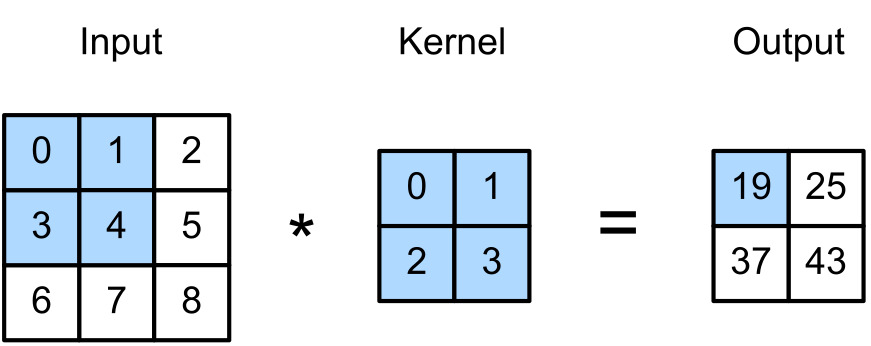
\includegraphics[width=\linewidth, height=2cm, keepaspectratio]{Pictures/convolutional-neural-network/Cross-Correlation-Operation.jpg}
            \caption*{$0\times0+1\times1+3\times2+4\times3=19$ $s=1, p=0$ \cite{dnn-1}}
        \end{figure}
    \end{minipage}
    \hfill
    \begin{minipage}{0.3\linewidth}
        \begin{figure}[H]
            \centering
            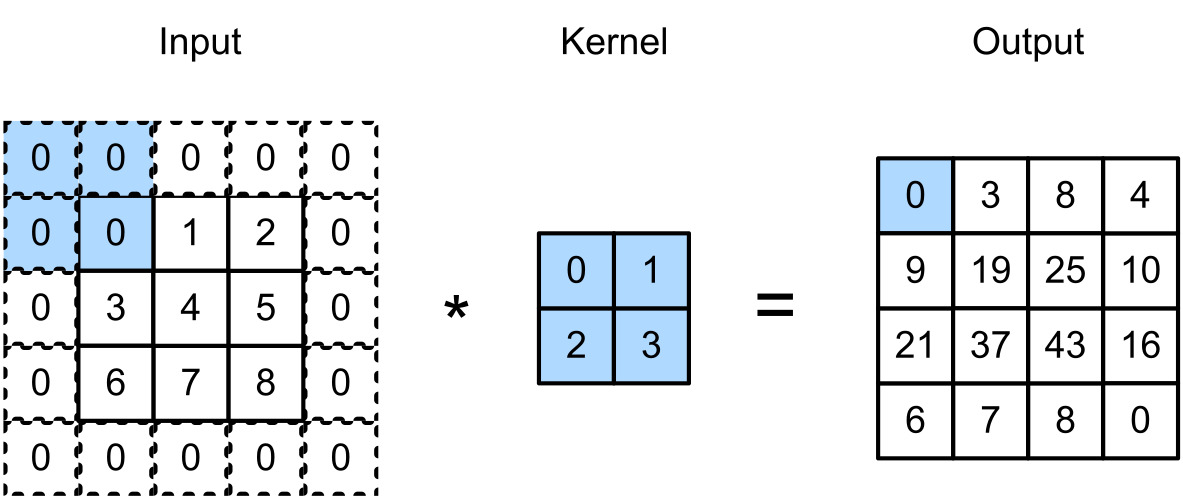
\includegraphics[width=\linewidth, height=2cm, keepaspectratio]{Pictures/convolutional-neural-network/conv-pad.jpg}
            \caption*{cross-correlation with padding $p_h=p_w=1$ \cite{dnn-1}}
        \end{figure}
    \end{minipage}
    \hfill
    \begin{minipage}{0.3\linewidth}
        \begin{figure}[H]
            \centering
            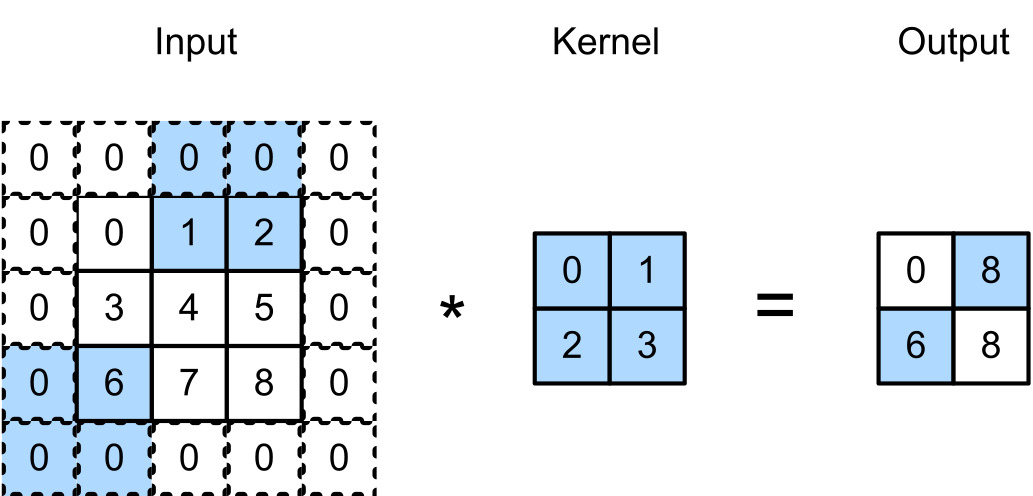
\includegraphics[width=\linewidth, height=2cm, keepaspectratio]{Pictures/convolutional-neural-network/conv-stride.jpg}
            \caption*{Cross-correlation with strides of $s_h=3$ and $s_w=2$ for height and width, respectively \cite{dnn-1}}
        \end{figure}
    \end{minipage}
\end{table}


\subsection{Multiple Input and Multiple Output Channels \cite{dnn-1}}

\begin{table}[H]
    \begin{minipage}[b]{0.65\linewidth}
        \begin{figure}[H]
            \centering
            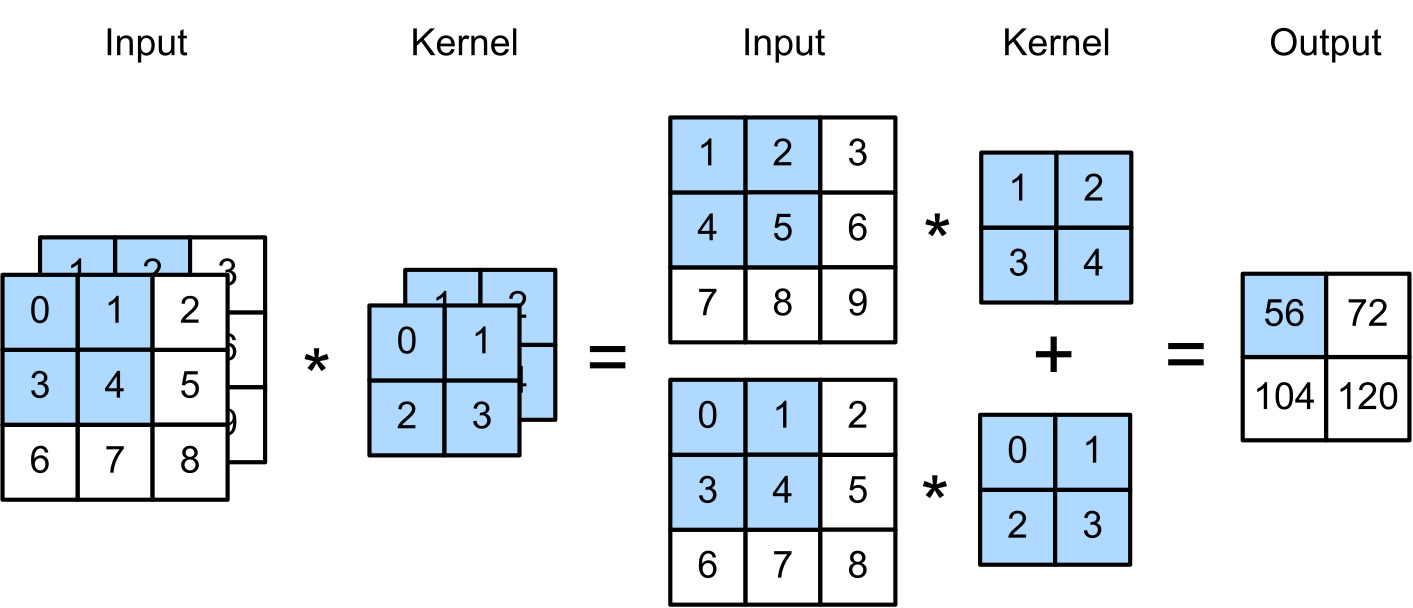
\includegraphics[width=\linewidth, height=3cm, keepaspectratio]{Pictures/convolutional-neural-network/conv-multi-in.jpg}
            \caption*{Cross-correlation computation with multiple (2) input channels}
            \caption*{$(1\times1+2\times2+4\times3+5\times4)+(0\times0+1\times1+3\times2+4\times3)=56$}
        \end{figure}
    \end{minipage}
    \hfill
    \begin{minipage}[b]{0.35\linewidth}
        \begin{figure}[H]
            \centering
            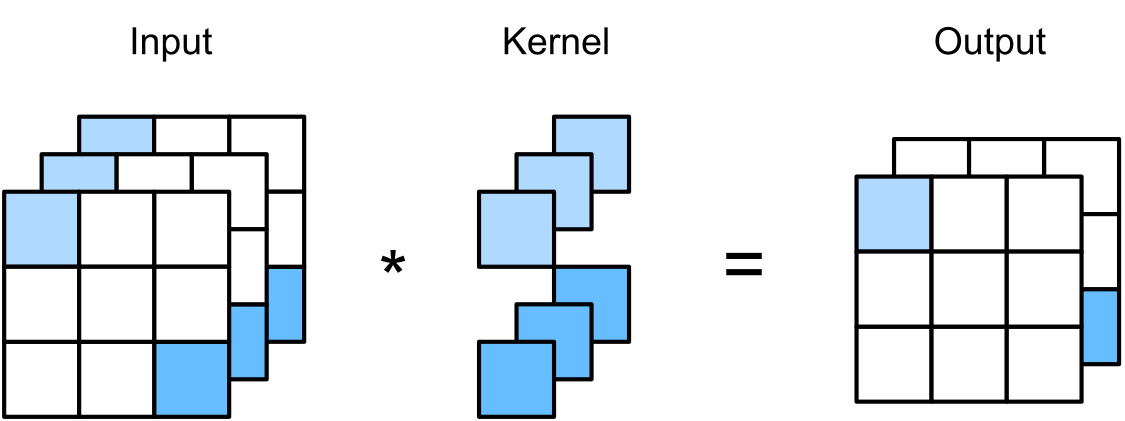
\includegraphics[width=\linewidth, height=3cm, keepaspectratio]{Pictures/convolutional-neural-network/conv-1x1.jpg}
            \caption*{Cross-correlation computation with multiple (3) input channels and multiple (2) output channels ($1\times 1$ Convolutional)}
            \caption*{$k_\textrm{h} = k_\textrm{w} = 1$}
        \end{figure}
    \end{minipage}
\end{table}

\begin{enumerate}
    \item When the \textbf{input data contains multiple channels}, we need to construct a convolution kernel with the same number of input channels as the input data, so that it can perform cross-correlation with the input data.

    \item To get an \textbf{output with multiple channels}, we can create a kernel tensor of shape $c_\textrm{i}\times k_\textrm{h}\times k_\textrm{w}$ for \textbf{every} output channel.\\
    We concatenate them on the output channel dimension, so that the shape of the convolution kernel is $c_\textrm{o}\times c_\textrm{i}\times k_\textrm{h}\times k_\textrm{w}$. \\
    In cross-correlation operations, the result on each output channel is calculated from the convolution kernel corresponding to that output channel and takes input from all channels in the input tensor.
\end{enumerate}



%%%%%%%%%%%%%%%%%%%%%%%%%%%%%%%%%%%%%%%%%%%%%%%%%%%%%%%%%%%%

\section{MLP Convolutional (mlpconv) Layer \cite{medium/towardsdatascience.com/review-nin-network-in-network-image-classification-69e271e499ee}}

\begin{figure}[H]
    \centering
    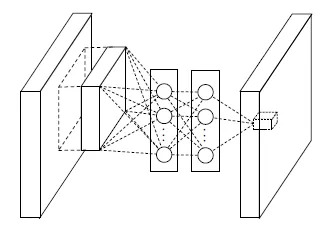
\includegraphics[width=\linewidth, height=3cm, keepaspectratio]{Pictures/layers/conv-layer-mlp.jpg}
    \caption{MLP Convolutional (mlpconv) Layer}
\end{figure}



%%%%%%%%%%%%%%%%%%%%%%%%%%%%%%%%%%%%%%%%%%%%%%%%%%%%%%%%%%%%

\section{Pooling Layer \cite{gfg-convolutional-neural-network-cnn-in-machine-learning,dnn-1}}\label{nn: Pooling Layer}

\begin{enumerate}
    \item[] output dimensions: 
    $
        \hfill
        n^{out}_h=\dfloor{\dfrac{n_\textrm{h}-k_\textrm{h}+p_\textrm{h}+s_\textrm{h}}{s_\textrm{h}}}
        \hfill 
        n^{out}_w=\dfloor{\dfrac{n_\textrm{w}-k_\textrm{w}+p_\textrm{w}+s_\textrm{w}}{s_\textrm{w}}}
        \hfill
        \text{\cite{dnn-1}}
    $
    
    \item default: $s=k$, so that pooling windows dont overlap

    \item Pooling layers \textbf{downsample} the spatial dimensions of the input, reducing the computational complexity and the number of parameters in the network. 
    
    \item Max pooling is a common pooling operation, selecting the maximum value from a group of neighboring pixels.

    \item unlike the cross-correlation computation of the inputs and kernels in the convolutional layer, the pooling layer contains no parameters (\textbf{there is no kernel})

    \item pooling operators are deterministic

    \item Pooling has \textbf{no model parameters}

    \item The pooling layer pools each input channel \textbf{separately}, rather than summing the inputs up over channels as in a convolutional layer.\\
    This means that the number of output channels for the pooling layer is the same as the number of input channels.
\end{enumerate}

%%%%%%%%%%%%%%%%%%%%%

\subsection{Max Pooling \cite{gfg-cnn-introduction-to-pooling-layer,dnn-1}} \label{cnn: Max Pooling}

\begin{enumerate}
    \item Max pooling is a pooling operation that selects the \textbf{maximum element} from the region of the feature map covered by the filter. 
    
    \item The output after max-pooling layer would be a feature map containing the \textbf{most prominent features} of the previous feature map.
\end{enumerate}

%%%%%%%%%%%%%%%%%%%

\subsection{Average Pooling \cite{gfg-cnn-introduction-to-pooling-layer,dnn-1}} \label{cnn: Average Pooling}
\begin{enumerate}
    \item Average pooling computes the \textbf{average of the elements} present in the region of feature map covered by the filter.
    
    \item Average pooling gives the average of features present in a patch.
\end{enumerate}

%%%%%%%%%%%%%%%%%%

\subsection{Global Pooling \cite{gfg-cnn-introduction-to-pooling-layer,dnn-1}} \label{cnn: Global Pooling}
\begin{enumerate}
    \item Global pooling reduces each channel in the feature map to a single value.
    
    \item Thus, an $n_h \times n_w \times n_c$ feature map is reduced to $1 \times 1 x nc$ feature map. 

    \item This is equivalent to using a filter of dimensions $n_h \times n_w$ i.e. the dimensions of the feature map.
\end{enumerate}

\begin{table}[h]
    \begin{minipage}[b]{0.32\linewidth}
        \begin{figure}[H]
            \centering
            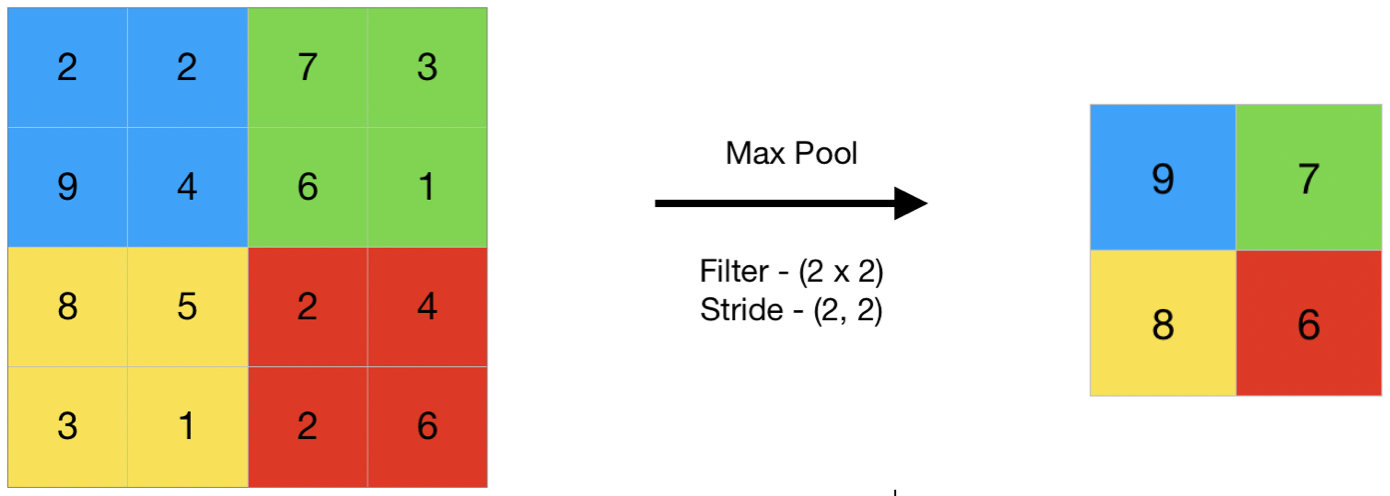
\includegraphics[width=\linewidth, height=4cm, keepaspectratio]{Pictures/convolutional-neural-network/pooling-max.png}
            \caption{Max Pooling}
        \end{figure}
    \end{minipage}
    \hfill
    \begin{minipage}[b]{0.32\linewidth}
        \begin{figure}[H]
            \centering
            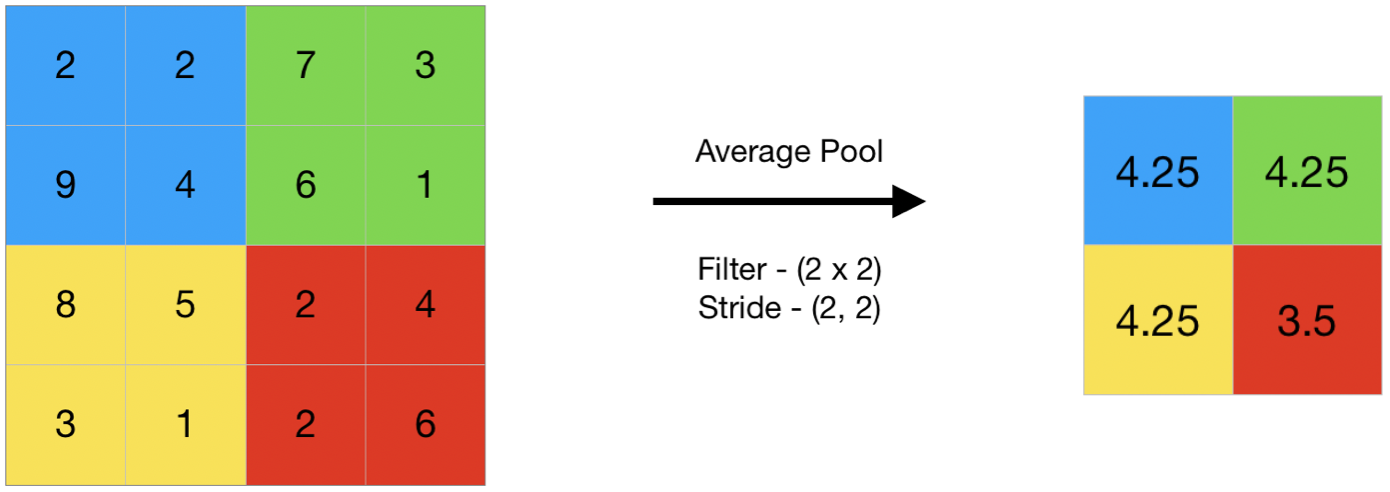
\includegraphics[width=\linewidth, height=4cm, keepaspectratio]{Pictures/convolutional-neural-network/pooling-average.png}
            \caption{Average Pooling}
        \end{figure}
    \end{minipage}
    \hfill
    \begin{minipage}[b]{0.32\linewidth}
        \begin{figure}[H]
            \centering
            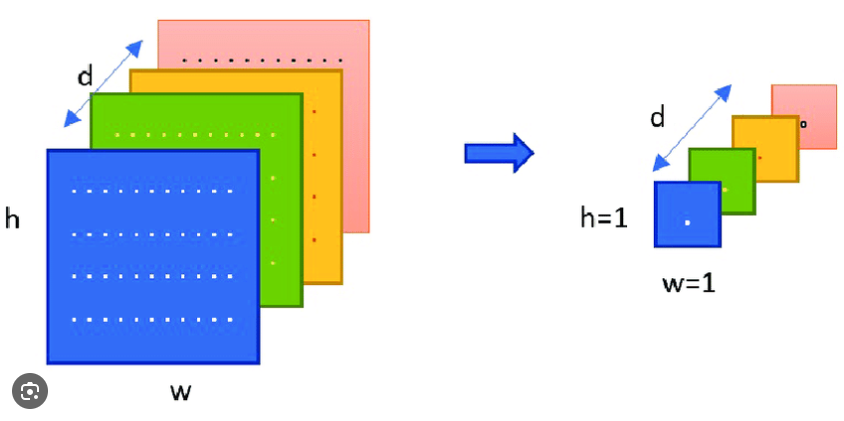
\includegraphics[width=\linewidth, height=4cm, keepaspectratio]{Pictures/convolutional-neural-network/pooling-global.png}
            \caption{Global Pooling}
        \end{figure}
    \end{minipage}
\end{table}


\subsection{Spatial Pyramid Pooling (SPP) Layer/ spatial pyramid matching (SPM) Layer \cite{arxiv/1406.4729-sppnet}}\label{Spatial Pyramid Pooling (SPP) Layer/ spatial pyramid matching (SPM) Layer}

\begin{enumerate}
    \item The SPP layer pools the features and generates fixed-length outputs, which are then fed into the fully-connected layers (or other classifiers).

    \item we perform some \textbf{information “aggregation”} at a deeper stage of the network hierarchy (between convolutional layers and fully-connected layers) to avoid the need for cropping or warping at the beginning.

    \item  It partitions the image into divisions from finer to coarser levels, and aggregates local features in them.

    
\end{enumerate}



\subsection{Region of Interest (ROI) Pooling Layer \cite{arxiv/1504.08083-fast-rcnn}}\label{cnn: Region of Interest (ROI) Pooling Layer}

\begin{enumerate}
    \item The RoI pooling layer uses max pooling to convert the features inside any valid region of interest into a small feature map with a fixed spatial extent of $H \times W$ (e.g., $7 \times 7$), where $H$ and $W$ are layer \textbf{hyper-parameters} that are \textbf{independent} of any particular RoI.

    \item Each RoI is defined by a four-tuple $(r, c, h, w)$ that specifies its top-left corner $(r, c)$ and its height and width $(h, w)$.

    \item RoI max pooling works by dividing the $h \times w$ RoI window into an $H \times W$ grid of sub-windows of approximate size ${\displaystyle \dfrac{h}{H} \times \dfrac{w}{W}}$ and then \textbf{max-pooling} (SEE: \fullref{cnn: Max Pooling}) the values in each sub-window into the corresponding output grid cell.

    \item Pooling is applied \textbf{independently} to each feature map channel, as in standard max pooling. 

    \item Special case of \fullref{Spatial Pyramid Pooling (SPP) Layer/ spatial pyramid matching (SPM) Layer}
\end{enumerate}

%%%%%%%%%%%%%%%%%%%%%%%%%%%%%%%%%%%%%%%%%%%%%%%%%%%%%%%%%%%%%%

\section{Dropout Layer}\label{nn: Dropout Layer}

SEE: \fullref{Dropout}



%%%%%%%%%%%%%%%%%%%%%%%%%%%%%%%%%%%%%%%%%%%%%%%%%%%%%%%%%%%%%%


\section{Flatten Layer \cite{gfg/what-is-a-neural-network-flatten-layer}}\label{Flatten Layer}

\begin{enumerate}
    \item A neural network flatten layer is used to convert the multi-dimensional output from the previous layer into a \textbf{one-dimensional array}, typically before feeding it into a fully connected layer for further processing.

    
\end{enumerate}


%%%%%%%%%%%%%%%%%%%%%%%%%%%%%%%%%%%%%%%%%%%%%%%%%%%%%%%%%%%%%%

\section{Activation Layer}
\textbf{SEE}: \fullref{chapter: Activation Functions}


%%%%%%%%%%%%%%%%%%%%%%%%%%%%%%%%%%%%%%%%%%%%%%%%%%%%%%%%%%%%%%

\section{Batch Normalization Layer (2015) \cite{dnn-1,arxiv/1502.03167-batch-normalization}} \label{Batch Normalization Layer}

\subsection{Batch Normalization \cite{dnn-1}} \label{Batch Normalization}

\begin{customTableWrapper}{1.5}
\begin{longtable}{l p{8cm}}
    $\boldsymbol{\mu}$ & mean \\
    $\boldsymbol{\Sigma}$ & variance \\
    $\mathcal{B}$ & minibatch \\
    $\mathbf{x} \in \mathcal{B}$ & input to batch normalization \\
    $\hat{\boldsymbol{\mu}}_\mathcal{B}$ & sample mean of $\mathcal{B}$ \\
    $\hat{\boldsymbol{\sigma}}_\mathcal{B}$ & sample standard deviation of $\mathcal{B}$ \\
    $\boldsymbol{\gamma}$ & scale parameter \\
    $\boldsymbol{\beta}$ & shift parameter \\
    $\epsilon > 0$ & small constant \\
\end{longtable}
\end{customTableWrapper}


\begin{enumerate}[itemsep=0.1cm]
    \item[] 
    $
        \hfill
        \textrm{BN}(\mathbf{x}) = \boldsymbol{\gamma} \odot \dfrac{\mathbf{x} - \hat{\boldsymbol{\mu}}_\mathcal{B}}{\hat{\boldsymbol{\sigma}}_\mathcal{B}} + \boldsymbol{\beta}
        \hfill
        \hat{\boldsymbol{\mu}}_\mathcal{B} = \dfrac{1}{|\mathcal{B}|} \dsum_{\mathbf{x} \in \mathcal{B}} \mathbf{x}
        \hfill
        \hat{\boldsymbol{\sigma}}_\mathcal{B}^2 = \dfrac{1}{|\mathcal{B}|} \dsum_{\mathbf{x} \in \mathcal{B}} (\mathbf{x} - \hat{\boldsymbol{\mu}}_{\mathcal{B}})^2 + \epsilon
        \hfill
    $

    \item BN a popular and effective technique that consistently accelerates the convergence of deep networks

    \item data preprocessing
    \begin{enumerate}
        \item first step is to \textbf{standardize} our input features to have zero mean $\boldsymbol{\mu} = 0$ and unit variance $\boldsymbol{\Sigma} = \boldsymbol{1}$ across multiple observations, frequently rescaling the latter so that the diagonal is unity, i.e., $\Sigma_{ii} = 1$

        \item another strategy is to rescale vectors to unit length, possibly zero mean per observation\\
        This can work well, e.g., for spatial sensor data.

    \end{enumerate}

    \item Standardizing vectors also has the nice side-effect of constraining the function complexity of functions that act upon it.

    \item for a typical MLP or CNN, as we train, the variables in intermediate layers (e.g., affine transformation outputs in MLP) may take values with widely varying magnitudes: whether along the layers from input to output, across units in the same layer, and over time due to our updates to the model parameters.\\
    drift in the distribution of such variables could hamper the convergence of the network.\\
    The alternative is to prevent the problem from occurring, simply by adaptive normalization.

    \item batch normalization conveys all three benefits: preprocessing, numerical stability, and regularization.

    \item Batch normalization is applied to individual layers, or optionally, to all of them: In each training iteration, we first normalize the inputs (of batch normalization) by subtracting their mean and dividing by their standard deviation, where both are estimated based on the statistics of the current minibatch.

    \item we apply a scale coefficient and an offset to recover the lost degrees of freedom. It is precisely due to this normalization based on batch statistics that batch normalization derives its name.

    \item if we tried to apply batch normalization with minibatches of size 1, we would not be able to learn anything. That is because after subtracting the means, each hidden unit would take value 0.

    \item when applying batch normalization, the choice of batch size is even more significant than without batch normalization, or at least, suitable calibration is needed as we might adjust batch size.

    \item After applying standardization, the resulting minibatch has zero mean and unit variance.\\
    The choice of unit variance (rather than some other magic number) is arbitrary.

    \item The estimates $\hat{\boldsymbol{\mu}}_\mathcal{B}$ and ${\hat{\boldsymbol{\sigma}}_\mathcal{B}}$ counteract the scaling issue by using noisy estimates of mean and variance.

    \item During training, exact calculation of mean and variance of entire dataset is \textbf{infeasible} because the intermediate variables for all data examples change every time we update our model.\\
    However, once the model is trained, we can calculate the means and variances of each layer’s variables based on the entire dataset.\\
    Indeed this is standard practice for models employing batch normalization; thus batch normalization layers function differently in training mode (normalizing by minibatch statistics) than in prediction mode (normalizing by dataset statistics).

    \item batch normalization typically behaves differently in training mode than in prediction mode
    \begin{enumerate}
        \item the noise in the sample mean and the sample variance arising from estimating each on minibatches is no longer desirable once we have trained the model

        \item we might not have the luxury of computing per-batch normalization statistics. \\
        For example, we might need to apply our model to make one prediction at a time.

    \end{enumerate}

    \item Typically, after training, we use the entire dataset to compute stable estimates of the variable statistics and then fix them at prediction time.

\end{enumerate}


\subsection{Batch Normalization and Fully Connected \cite{dnn-1}}

\begin{enumerate}[itemsep=0.2cm]
    \item When applying batch normalization to fully connected layers, Ioffe and Szegedy (2015), in their original paper inserted batch normalization after the affine transformation and before the nonlinear activation function. 

    \item[] 
    $
        \hfill
        \mathbf{h} = \phi(\textrm{BN}(\mathbf{W}\mathbf{x} + \mathbf{b}) )
        \hfill
    $
    
    \item Later applications experimented with inserting batch normalization right after activation functions.
    
    \item[] $
        \hfill
        \mathbf{h} = \textrm{BN}(\phi(\mathbf{W}\mathbf{x} + \mathbf{b}) )
        \hfill
    $

    \item mean and variance are computed on the same minibatch on which the transformation is applied
\end{enumerate}


\subsection{Batch Normalization and Convolutional Layer \cite{dnn-1}}

\begin{enumerate}
    \item with convolutional layers, we can apply batch normalization after the convolution but before the nonlinear activation function

    \item The key difference from batch normalization in fully connected layers is that we apply the operation on a \textbf{per-channel} basis across all locations

    \item Assume that our minibatches contain $m$ examples and that for each channel, the output of the convolution has height $h$ and width $w$. For convolutional layers, we carry out each batch normalization over the $m\cdot h\cdot w$ elements \textbf{per output channel} simultaneously. 
    
    \item we collect the values over all spatial locations when computing the mean and variance and consequently apply the same mean and variance within a given channel to normalize the value at each spatial location. 
    
    \item Each channel has its own scale and shift parameters, both of which are scalars.

    \item in the context of convolutions the batch normalization is well defined even for minibatches of size $1$: after all, we have all the locations across an image to average.\\
    Consequently, mean and variance are well defined, even if it is just within a single observation.
\end{enumerate}


\subsection{Layer Normalization \cite{dnn-1}}

\begin{enumerate}[itemsep=0.15cm]
    \item It works just like a batch norm, only that it is applied to \textbf{one observation} at a time. 
    
    \item Both the offset and the scaling factor are scalars.

    \item For an $n$-dimensional vector $\mathbf{x}$, layer norms are given by
    
    \item[] $
        \hfill
        \mathbf{x} \rightarrow \textrm{LN}(\mathbf{x}) 
        =  \dfrac{\mathbf{x} - \hat{\mu}}{\hat\sigma}
        \hfill
        \hat{\mu} \stackrel{\textrm{def}}{=} \dfrac{1}{n} \dsum_{i=1}^n x_i
        \hfill
        \hat{\sigma}^2 \stackrel{\textrm{def}}{=} \dfrac{1}{n} \dsum_{i=1}^n (x_i - \hat{\mu})^2 + \epsilon
        \hfill
        (\epsilon > 0)
    $

    \item it prevents divergence

    \item the output of the layer normalization is scale independent\\
    That is, we have $\textrm{LN}(\mathbf{x}) \approx \textrm{LN}(\alpha \mathbf{x})$ for any choice of $\alpha \neq 0$.\\
    This becomes an equality for $|\alpha| \to \infty$ (the approximate equality is due to the offset $\epsilon$ for the variance).


\end{enumerate}































































